\section{Introduction}
\label{sec:intro}

Autoregressive (AR) language models generate text one token at a time;
each token requires a forward pass over the growing KV cache.
Block-diffusion models generate an entire block of tokens in parallel
through iterative denoising, then step to the next block. The structural
difference produces different cost shapes, and the shapes determine which
architecture is faster for a given workload.

We measure both on a pinned stack --- vLLM \vllmVersion{}, \gpuModel{},
BF16 --- for structured log extraction from the LOGHUB BGL corpus. The
task is 12-field JSON extraction from log lines, scored on a 9-field
macro F1. The models are Qwen2.5-3B-Instruct (AR, 3.0\,B active) and
DiffusionGemma-26B-A4B (DG, 4.0\,B active of 26\,B total), matched on
active parameters. At $L{=}256$ output tokens they reach quality
equivalence:
\begin{equation}
\Delta_{\mathrm{F1}} = |\arThreeBFnine - \dgNineF| = \qualityGap, \quad
\text{95\% CI } [-0.012, +0.011], \quad n = 300
\end{equation}

Eight corrections --- five harness defects and three withdrawn claims ---
were made before this version. Five of the eight biased against the AR
arm (Appendix~\ref{app:defects}). All were found by re-reading committed
artifacts, not by running new experiments.

\paragraph{Numeric precision}

Every number in this paper is quoted to a precision its measurement error
supports. Latency is quoted to 0.1\,ms: the run-to-run CV on the pinned
stack is \arCV--\dgCV\%, so 0.1\,ms is real resolution at the p50. F1
scores are quoted to three decimals: at $n = \nPerCell$ events the
standard error of a nine-field macro F1 is roughly 0.006, so three
decimals is the defensible resolution; differences below 0.006 (e.g.,
0.852 vs 0.855 in Table~\ref{tab:niche}) fall within the noise band and
are not statistically significant. Ratios and multipliers are quoted
to one decimal. Fitted coefficients are quoted only to the precision the
residuals support --- the K-sweep fit at $R^2 = \kfitRsq$
(Appendix~\ref{app:decomp}) is cited as a shape, not a measurement.

\begin{figure}[t]
\centering
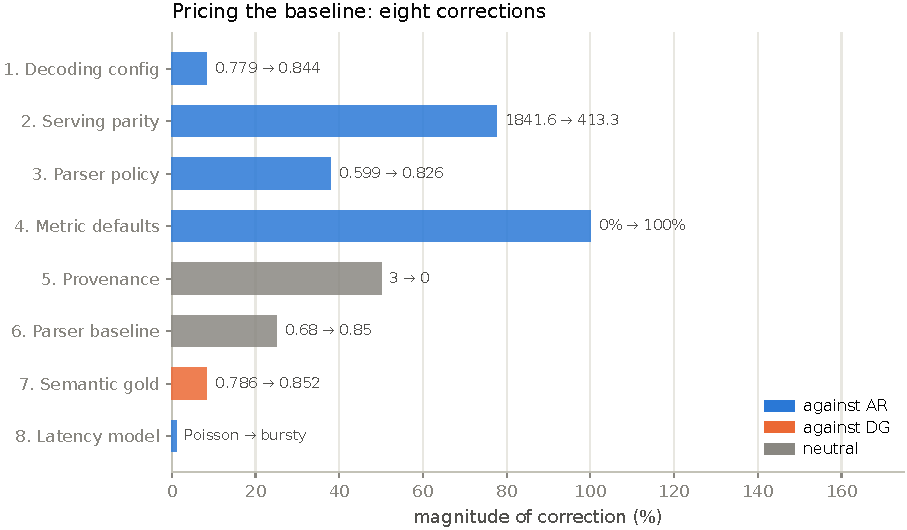
\includegraphics[width=\linewidth]{figures/fig8_defects.pdf}
\caption{Eight priced errors in our own comparison harness, each found by
re-reading committed artifacts (BGL, $n{=}300$ per cell, $K{=}8$). Five of eight
biased against the autoregressive arm. The clustering on one arm is
suggestive, though the sample ($n{=}8$) is too small for a statistical
claim.}
\label{fig:defects}
\end{figure}

\begin{table}[h]
\centering
\caption{The paper in one table. The diffusion model wins the latency
column and loses the deployment comparison behind it.}
\label{tab:summary}
\begin{tabularx}{\linewidth}{@{}L r r@{}}
\toprule
& \thead{\ARthree\,(active-param.)} & \thead{\DG-26B-A4B} \\
\midrule
\tabfont 9-field macro F1 ($L{=}\canvasLength$)      & \arThreeBFnine & \dgNineF \\
\tabfont Active parameters                            & 3.0\,B & 4.0\,B \\
\tabfont p50 latency at $L{=}\canvasLength$, batch-1  & \arAnchorTwoFive\,ms & \dgAnchorTwoFive\,ms \\
\tabfont Within-block marginal cost per token          & \arSlope\,ms & 0.0\,ms \\
\tabfont Block boundary cost (per \canvasLength\ tokens) & n/a & \dgStep\,ms \\
\tabfont Marginal cost per prompt token               & \arInputSlope\,ms & \dgInputSlope\,ms \\
\tabfont Batch-1 $\to$ peak throughput multiplier     & \arBatchLo--\arBatchHi$\times$ & $\leq$\dgBatchVllmHi$\times$ \\
\tabfont Energy per event, net of idle (AR-3B / DG)     & \arThreeEnergy\,J ($5.3\times$) & \dgEnergy\,J \\
\bottomrule
\end{tabularx}
\end{table}
